\documentclass{cmspaper}
\usepackage{graphicx}
\usepackage{rotate}
\usepackage{relsize}
\usepackage{lineno}

\newcommand{\met} {\ensuremath{E\!\!\!\!/_T}}
\newcommand{\ttbar} {\ensuremath{t\bar{t}~}}
\newcommand{\ptll} {\ensuremath{P_T(\ell\ell)}}
\newcommand{\ptllres} {\ensuremath{P^{\rm res}_T(\ell\ell)}}
\def\ack{\section*{Acknowledgments}}

\linenumbers


\begin{document}

%==============================================================================
% title page for many authors
%
\begin{titlepage}
\title{Inclusive search for Same-Sign Top Quark Pair Production using di-leptons at $\sqrt{s} = 7 $ TeV}

  \begin{Authlist}
    D.~ Barge, C.~Campagnari, P.~Kalavase, D.~Kovalskyi, V.~Krutelyov, J.~Ribnik
    \Instfoot{ucsb}{University of California, Santa Barbara}
    W.~Andrews, G.~Cerati, D.~Evans, F.~Golf, S.~Padhi, Y.~Tu, F.~W\"urthwein, A.~Yagil, J.~Yoo
    \Instfoot{ucsd}{University of California, San Diego}
    L.~Bauerdick, I.~Bloch, K.~Burkett, I.~Fisk, Y.~Gao, O.~Gutsche, B.~Hooberman
    \Instfoot{fnal}{Fermi National Accelerator Laboratory, Batavia, Illinois}
  \end{Authlist}

\begin{abstract}
Significant evidence of asymmetries in $t\bar{t}$ productions have been recently reported by the Tevatron experiments. 
This could imply an enhancement of  same-sign top pair production via non-universal massive neutral vector boson ($Z'$) at the LHC. 
This note presents the first inclusive search for same-sign top quark pair production using di-leptons at the LHC. 
The study is performed using data corresponding to an integrated luminosity of 35 pb$^{-1}$ at $\sqrt{s} = 7 $ TeV recorded  by CMS in 2010. 
No excess above the standard model background expectation is observed. Limits at 95\% confidence level are set 
on the propagator mass as a function of $Z'$ couplings to the standard model quarks. 
\end{abstract}
\end{titlepage}

\section{Introduction}
\label{sec:intro}
The LHC has recently started delivering proton-proton collisions at a centre-of-mass energy of 7 TeV. 
Physics analyses at the LHC frequently depend on various inputs from theory that are only known with
limited accuracy. An important parameter to compare simulations and data is the predicted cross section for the former. The cross section calculations depend on various orders of perturbation theory
as well as the determination of PDFs. 

Most often there is no unique choice of which prescription should be used in 
a given analysis when comparing the simulations to the data. This study aims at establishing a convention as well 
as a certain set of choices based on inputs from the Monte Carlo simulations that are currently being used in the 
CMS collaboration. The higher order cross sections are then computed using these choices, and  
uncertanities due to the underlining assumptions are also computed.

In Section~\ref{sec:normalization}, guidelines for the calculation of K-factors based on higher order cross sections
along with given scales and PDF uncertainties are provided. In Section~\ref{sec:assumptions}
the assumptions made for these calculations are given, followed by the results in Section~\ref{sec:results}
and finally, in Section~\ref{sec:conclusion} we summarize the results.  

%%% commented out - DLE
%%%\section{Data Samples}
\label{sec:datasamples}
This study is based on the 3\_1\_X reco full simulation SM background samples
listed in Table~\ref{tab:datasets}.  The Standard Model (SM) data sets have been normalized 
to the cross-sections~\cite{mcsusy};  for the SUSY parameter scan studies, we have used  
3\_3\_6 reco fast simulation data set~\cite{fast10}. In this data set several benchmark 
point are produced using fixed $A_0 = 0 $, tan$\beta = 3$, sign $\mu > 0 $ but with varying 
$m_{0} (0 - 2000)$ and $m_{1/2} (100 - 600)$ on a grid of 50 and 20 GeV steps, respectively.

\begin{table}[hbt]
\begin{center}
\begin{tabular}{|l|}\hline
{\tt /WW/Summer09-MC\_31X\_V3\_7TeV-v1/GEN-SIM-RECO} \\
{\tt /WZ/Summer09-MC\_31X\_V3\_7TeV-v1/GEN-SIM-RECO} \\
{\tt /ZZ/Summer09-MC\_31X\_V3\_7TeV-v1/GEN-SIM-RECO} \\
{\tt /Wenu/Summer09-MC\_31X\_V3\_7TeV-v1/GEN-SIM-RECO} \\
{\tt /Wmunu/Summer09-MC\_31X\_V3\_7TeV-v1/GEN-SIM-RECO} \\
{\tt /Wtaunu/Summer09-MC\_31X\_V3\_7TeV-v1/GEN-SIM-RECO} \\
{\tt /Zee/Summer09-MC\_31X\_V3\_7TeV-v1/GEN-SIM-RECO} \\
{\tt /Zmumu/Summer09-MC\_31X\_V3\_7TeV-v1/GEN-SIM-RECO} \\
{\tt /Ztautau/Summer09-MC\_31X\_V3\_7TeV-v1/GEN-SIM-RECO} \\
{\tt /TTbar/Summer09-MC\_31X\_V3\_7TeV-v1/GEN-SIM-RECO} \\
{\tt /SingleTop\_sChannel-madgraph/Summer09-MC\_31X\_V3\_7TeV-v1/GEN-SIM-RECO} \\
{\tt /SingleTop\_tChannel-madgraph/Summer09-MC\_31X\_V3\_7TeV-v1/GEN-SIM-RECO} \\
{\tt /SingleTop\_tWChannel-madgraph/Summer09-MC\_31X\_V3\_7TeV-v1/GEN-SIM-RECO} \\
{\tt /TANB3\_CMSW336FASTv0JetID/spadhi-TANB3\_CMSW336FASTv0JetID-*/USER} \\
\hline
\end{tabular}
\caption{The data sets used in this study.\label{tab:datasets}}
\end{center}
\end{table}

The Monte Carlo events were analyzed with CMSSW\_3\_3\_6 
with the additional tags listed in Table~\ref{tab:tags}.

\begin{table} [htb]
\begin{center} 
\begin{tabular}{|l|} \hline
{V00-03-04 RecoEgamma/EgammaTools} \\
{V03-00-12-13 RecoMET/METProducers} \\
{V00-02-07-15 RecoMET/METAlgorithms} \\
{V00-06-10-02 RecoMET/Configuration} \\
{V03-01-01-04 DataFormats/METReco} \\
{V00-05-38 RecoEcal/EgammaCoreTools} \\
{V01-08-23-05 JetMETCorrections/Configuration} \\
{V01-08-08-09 CondFormats/JetMETObjects} \\
{V02-06-03 HLTrigger/HLTcore} \\
\hline
\end{tabular}
\caption{Additional software tags used in this study.\label{tab:tags}}
\end{center}
\end{table}

%%% commented out - DLE
%%%\section{Event Selection}
\label{sec:eventselection}

The event selection used is not optimized for any specific SUSY scenario.
It is based on small modifications to the dilepton event selections 
that we used in recently approved 
$WW$\cite{ww} and \ttbar\cite{ttbar} cross-section
analyses.  A quick summary of the event selection is:
\begin{itemize}
\item The event is required to pass the single $e$ or $\mu$  triggers.
\item Two isolated, same or opposite sign leptons ($ee$, $e\mu$, and $\mu\mu$). 
\item Leptons must have $P_T > 10$ GeV, $|\eta|< 2.4$ and at least one of them must have $P_T > 20$ GeV.
\item For SS analyses, we veto the candidate lepton, if an extra lepton in the event, pairs with the candidate lepton
to form a $Z$ within the mass range between $76 < m_{\ell\ell} $ (GeV) $< 106$. This requirement is 
designed to reject $WZ$ events.
\item At least three L2L3 corrected caloJets with $P_T > 30$ GeV and $|\eta|< 2.4$.
\item The scalar sum of the $P_T$ of all jets passing the requirements above should be $>$ 200 GeV.
\item We require \met~$>$ 80 GeV. 
\item -------- NEED TO OUTLINE THE OS SELECTION AS WELL HERE IN SOME DETAILS ----------
\end{itemize}
\noindent The details of the lepton and trigger selections are given below.

\subsection{Electron Selection}
\label{sec:electron}

\begin{itemize}
\item The electron ID is the ``e-gamma category based looseID''.
\item No muon candidate within $\Delta R < 0.1$.
\item $|d_0| < 200~\mu m$ (corrected for beamspot).
\item Iso $<$ 0.1, where Iso=Sum/Max(20 GeV, $P_T$), and Sum = tkIso + hcalIso +  Max(0 GeV, ecalIso - 2GeV).
All isolation sums are the standard sums used in release 3\_1\_X from the egamma group (cone of
0.4 for ecal, jurassic, rec-hit based; cone of 0.3 for tracker, and cone of 0.4 for hcal).
\item Conversion rejection~\cite{conversion} using tracks within cone of 0.3 of the candidate electron for SS studies: 
\begin{itemize}
\item $|\Delta \cot\theta| < 0.02$; the difference between cotangent polar angles of tracks parallel to 
each other.
\item $|d_{2d}| < 0.02$ cm; the two dimensional distance between points within nearest tracks.
\item The charge of the associated GSF and CTF tracks must be consistent.
If the CTF track is not reconstructed, the electron is kept.
\end{itemize} 
\end{itemize}

\subsection{Muon Selection}
\label{sec:muon}
\begin{itemize}
\item Must be a global muon {\bf and} a tracker muon~\cite{glbtrk}.
\item GlobalMuonPromptTight (global $\chi^2$/ndof$<$10)~\cite{muonid}.
\item At least 11 valid hits for the silicon track~\cite{muonid}.
\item $|d_0| < 200~\mu m$ (from silicon track, corrected for beamspot).
\item Global fits must have hits in the muon chambers.
\item Minimum ionizing: EcalVetoEnergy $<$ 4 GeV and HcalVetoEnergy $<6$ GeV~\cite{vplusj}. 
\item Iso $<$ 0.1, where Iso=Sum/Max(20 GeV, $P_T$), and Sum = tkIso + hcalIso +  ecalIso.
All isolation sums are the standard sums stored in the muon object in release 3\_1\_X, and
are calculated in a cone of 0.3.
\end{itemize}

\subsection{Trigger Selection}
\label{sec:trigger}
We use inclusive lepton triggers with no isolation, $i.e.$, the logical OR of {\tt HLT\_Ele15\_SW\_L1R} and {\tt HLT\_Mu9}.  
The combined trigger efficiency is $\sim 99$\% for dilepton events that pass the event selection.
These triggers are expected to be present in the data taking trigger table.

\section{Same Sign Dileptons}
\label{sec:samesign}

This section summarizes the results of the SUSY parameter space scan
in the same sign di-lepton channel. The measurement stratzgy is  
described in details in a CMS note~\cite{ssnote}. The technique
utilizes two data-driven methods to estimate background characterized
by the presence of two high $P_T$, isolated, same sign leptons,
$\met$, and significant hadronic activity.  For the purposes
of this note we restrict ourselves to the $ee$, $e\mu$, and $\mu\mu$
final states, {\em i.e.}, we do not consider $\tau$'s, except in the
case that the $\tau$ decays leptonically. 

As we will show in Section~\ref{sec:ssyields}, for a reasonable event
selection the main background is from \ttbar decays. The data-driven background 
prediction is based on a combination of estimating ``fake leptons''\cite{fakenote} (FakeRate) 
and electrons reconstructed with the wrong sign\cite{ssnote} (Charge FlipRate). The probability
for muons to be reconstructed with the wrong sign at the relevant momenta is negligible.

\subsection{Event Yields}
\label{sec:ssyields}

The expected SM event yields in 100~pb$^{-1}$ after applying the event selections
described in Section~\ref{sec:eventselection} to the data sets described in
Section~\ref{sec:datasamples} are detailed below

\begin{table}[hbt]
\begin{center}
%\small\addtolength{\tabcolsep}{-5pt}
\renewcommand{\arraystretch}{1.2}
 {\footnotesize
\begin{tabular}{|l|c|c|c|c|c|c|c|c|}\hline
Same Sign leptons & Total SM & \ttbar & Single top & WZ & ZZ & WW & DY & Wjets \\ \hline

$ee$ & 0.07$\pm$0.04 & 0.06$\pm$0.04 & 0.00$\pm$0.00 & 0.01$\pm$0.01 & 0.00$\pm$0.00 & 0.00$\pm$0.00 & 0.00$\pm$0.00 & 0.00$\pm$0.00 \\
$\mu\mu$ & 0.09$\pm$0.05 & 0.09$\pm$0.05 & 0.00$\pm$0.00 & 0.00$\pm$0.00 & 0.00$\pm$0.00 & 0.00$\pm$0.00 & 0.00$\pm$0.00 & 0.00$\pm$0.00 \\
$e\mu$ & 0.22$\pm$0.08 & 0.21$\pm$0.08 & 0.00$\pm$0.00 & 0.01$\pm$0.01 & 0.00$\pm$0.00 & 0.00$\pm$0.00 & 0.00$\pm$0.00 & 0.00$\pm$0.00 \\ 
total & 0.38$\pm$0.10 & 0.36$\pm$0.10 & 0.00$\pm$0.00 & 0.02$\pm$0.01 & 0.00$\pm$0.00 & 0.00$\pm$0.00 & 0.00$\pm$0.00 & 0.00$\pm$0.00 \\ \hline
\end{tabular} }
\caption{Expected number of SM events passing the event selection in 100 pb$^{-1}$ of integrated 
luminosity. Uncertainties are from MC statistics.\label{tab:ssyields}}
\end{center}
\end{table}

The dominant SM contribution is from \ttbar decays. The total estimated background 
is obtained after the application of Fake and Charge Flip rate to the entire ensamble
of SM samples. The results of the application of the procedure is summarized in Table~\ref{tab:sm_preditcion}.

\begin{table}[hbt]
\begin{center}
\begin{tabular}{|l|c|}\hline
Sample & Event yield \\ \hline
Total SM (Observed) & 0.38 $\pm$ 0.10 \\
Total SM (Predicted) & 0.36 \\
\hline
\end{tabular}
\caption{ Observed and predicted number of SM events passomg the event selection in 100 pb$^{-1}$ of integrated luminosity. The uncertainty is from Monte Carlo statistics.\label{tab:sm_preditcion}}
\end{center}
\end{table}

\subsection{Procedure for Determining $5\sigma$ Discovery Reach}
\label{sec:significance}

The $5\sigma$  discovery reach is estimated in the $m_{0}-m_{1/2}$
plane by  performing our analysis at each of the  mSUGRA scan points.
Expected event yield is determined based on the number of events passing
all cuts and scaled by the LO cross section for that point with 100/pb or 1/fb
of simulated events respectively . We apply both of the above mentioned data-driven 
estimation procedures to determine the ``signal contamination'' at each of the benchmark points. 
The significance if quantified by the observed yield and the predicted background
using estimators: $Z_{Bi}$~\cite{cite:cousins}  and $Z_{N}$\cite{cite:conway}. Following
are used in order to compute the significance.
\begin{itemize}
\item The predicted background yield
\item The relative systematic  uncertainty on the predicted background
yield (set to 50\%)
\item The  statistical uncertainty  on the predicted  background yield
($Z_N$ only, set to 0)
\item The observed yield
\end{itemize}
Figure~\ref{fig:ss_zn} and Figure~\ref{fig:ss_zbi} shows the discovery reach for various 
luminosity scenarios in one of the mSUGRA planes using $Z_{N}$ and $Z_{Bi}$ respectively.
Clearly, a large region of phase space can be accessed using higher luminosity. 
\vspace{3 mm}
\begin{figure}[htb]
\begin{center}
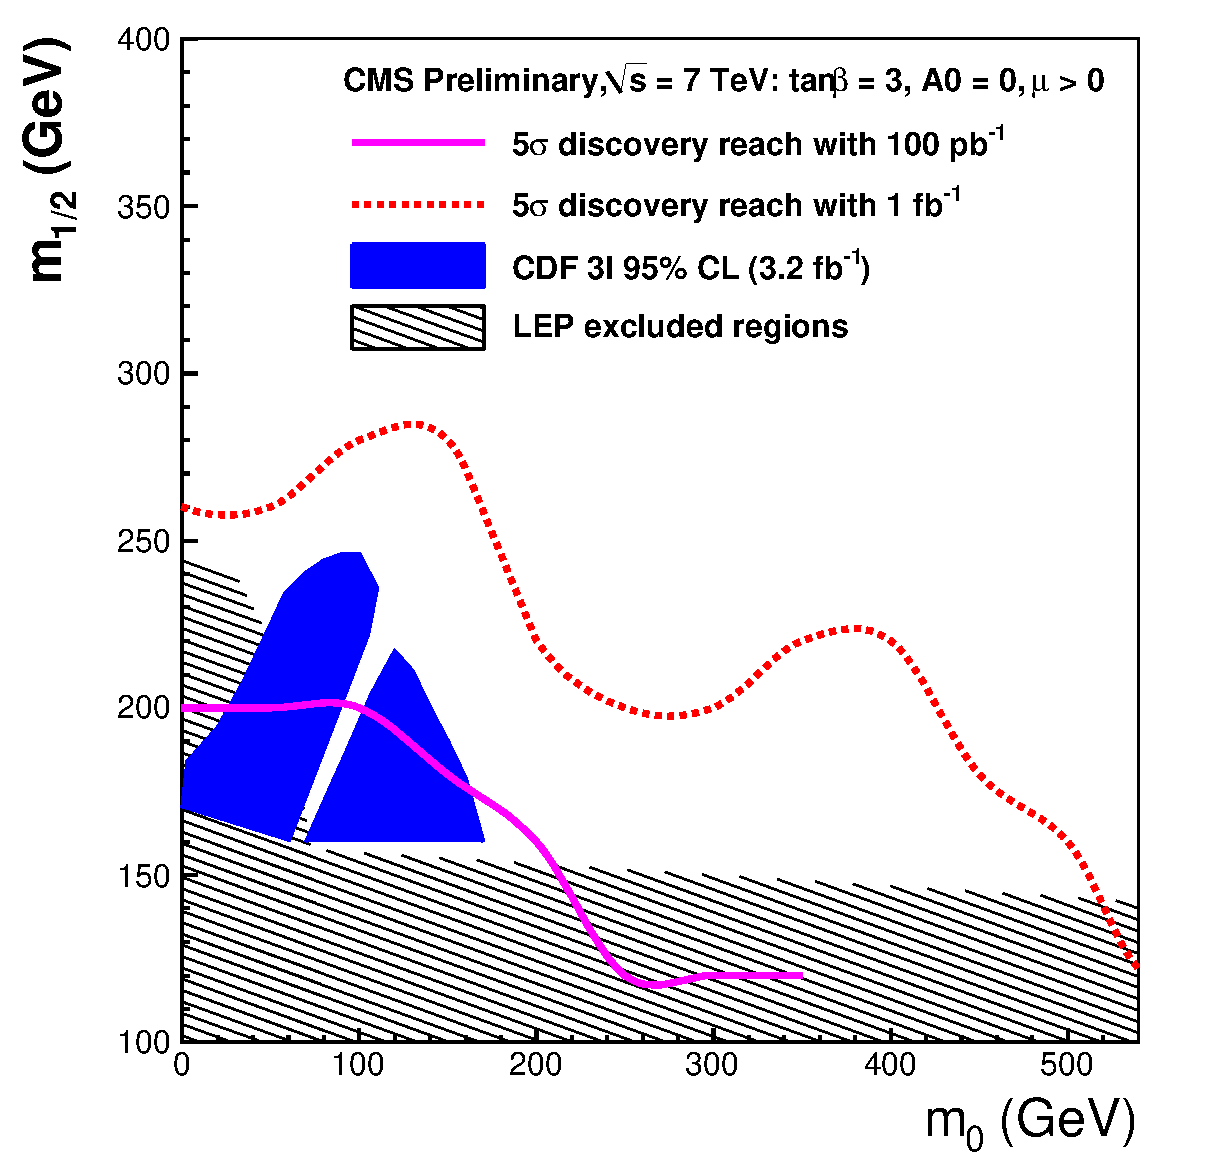
\includegraphics[width=0.7\linewidth]{figs/massreachss_zn.eps}
\caption{Discovery reach using significance estimated by $Z_N$~\cite{cite:conway} 
in the mSUGRA $m_{0}-m_{1/2}$ plane with tan$\beta = 3$, A$_0 = 0$, $\mu > 0$. 
Curves are shown for different luminosity scenario. The blue region was excluded by 
the CDF experiment [xx] and the black hashed region was excluded by the LEP 
experiments [xx].\label{fig:ss_zn}}
\end{center}
\end{figure}
\vspace{3 mm}
\begin{figure}[htb]
\begin{center}
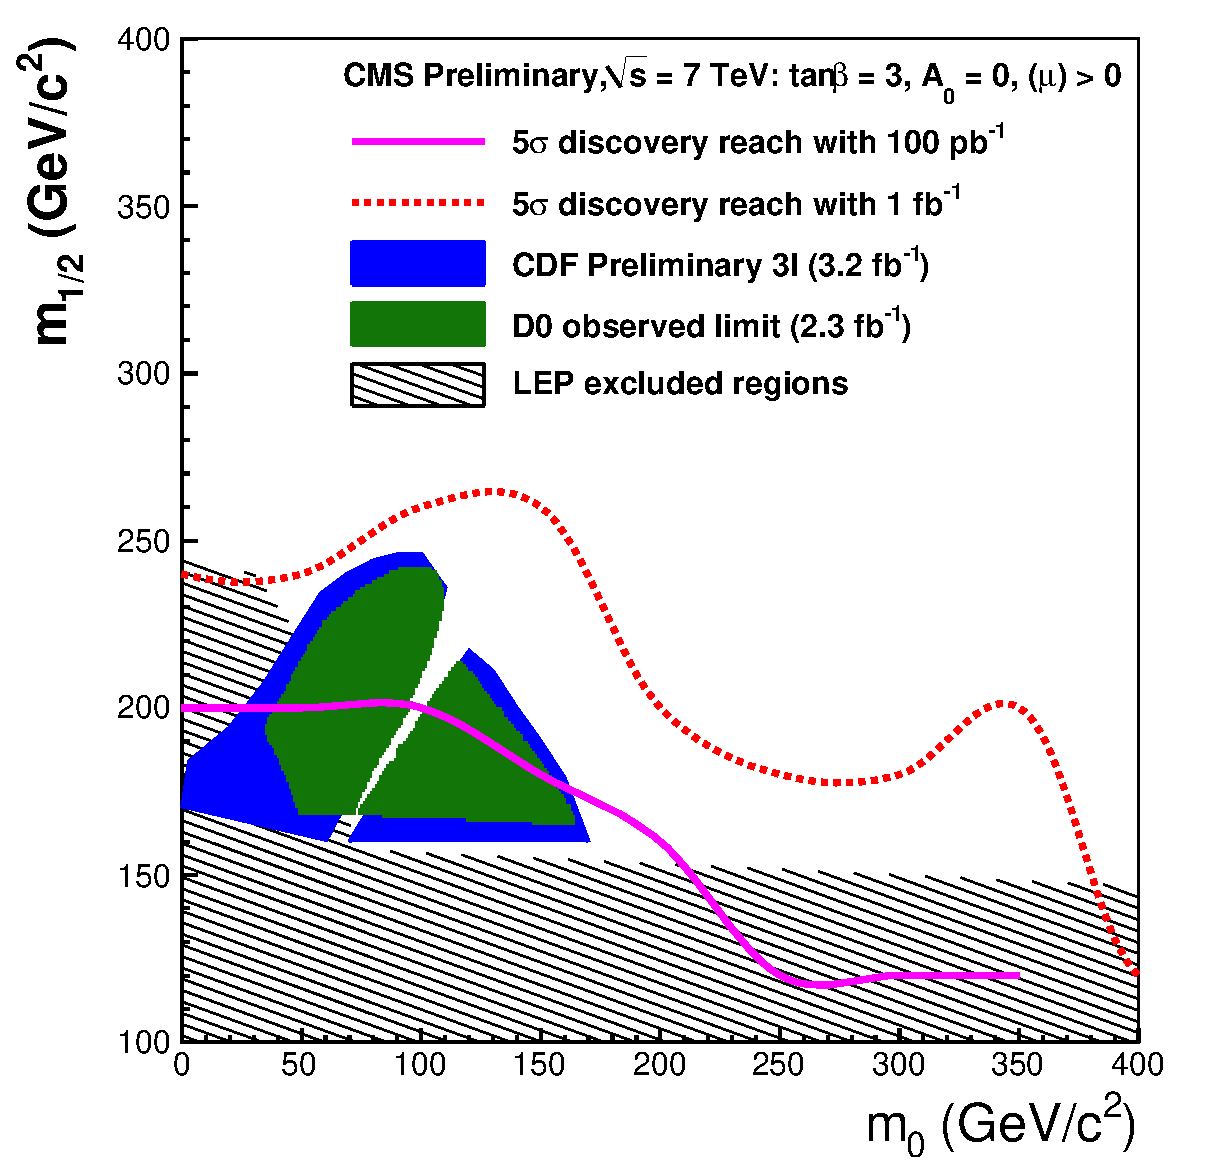
\includegraphics[width=0.7\linewidth]{figs/massreachss_bi.eps}
\caption{Discovery reach using significance estimated by $Z_{Bi}$~\cite{cite:cousins} 
in the mSUGRA $m_{0}-m_{1/2}$ plane with tan$\beta = 3$, A$_0 = 0$, $\mu > 0$. 
Curves are shown for different luminosity scenario. The blue region was excluded by 
the CDF experiment [xx] and the black hashed region was excluded by the LEP 
experiments [xx].\label{fig:ss_zbi}}
\end{center}
\end{figure}

\subsection{Procedure for Excluding a Region of the mSUGRA Parameter Space}
\label{sec:exclusion}

Next we  determine the region of  the mSUGRA parameter  space which we
expect  to exclude  at 95\%  confidence level  (CL) if  we see
the standard model (SM) expected yields in data. 
We  assume  that  we find  the  same
predicted background yield  and observed yield in data  that we expect
to  find based on  our SM  MC. However, as the latter is 0.4,
we work the math for both an observation of 0 or 1 events in 100/pb.
We  use this  information to  exclude a subset of the mSUGRA points using 
the following procedure.

The first  step is to  determine the 95\%  CL upper limit (UL)  on the
signal yield using a Bayesian  method from John Conway, implemented in
the program bayes.f. The required  inputs are: the observed yield, the
relative  uncertainty in  the  signal acceptance  (set  to 15\%),  the
predicted  background yield,  and  the total  error  on the  predicted
background yield. We assume $0.4 \pm 0.6$ for background yield and 
its uncertainty.
\vspace{3 mm}
\begin{figure}[htb]
\begin{center}

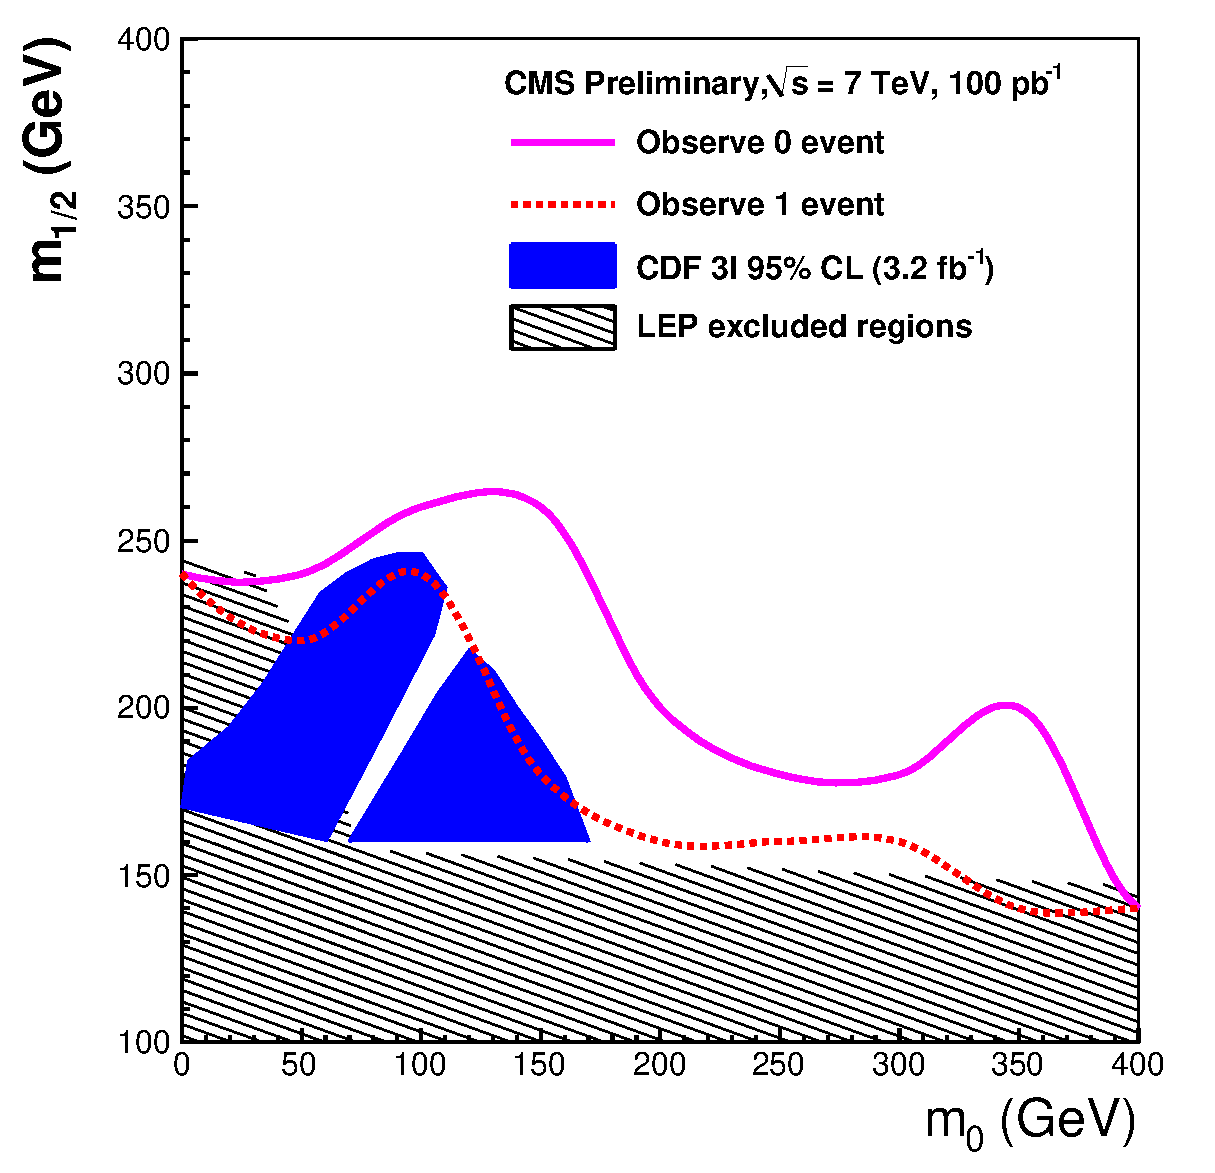
\includegraphics[width=0.485\linewidth]{figs/exclusion100ss.eps}
\includegraphics[width=0.485\linewidth]{figs/exclusion1fbss.eps}
\caption{ $m_{0}-m_{1/2}$ exclusion plot at the 95 \% C.L in the framework of 
mSUGRA assuming R-parity conservation using an  integrated  luminosity of  
$100~\mathrm{pb}^{-1}$ (left) and $1~\mathrm{fb}^{-1}$ (right). The blue region
was excluded by the CDF experiment [xx]. The black hashed region was excluded
by the LEP experiments [xx].\label{fig:ss_exclusion}}

\end{center}
\end{figure}

These values lead to 
to  95\% CL  ULs  of 3.2 and 4.7  signal  events respectively for an assumed 
observation of 0 or 1 events.

Next, we  wish to exclude mSUGRA  points based on the  signal yield UL
derived above.   The most obvious  way to do  so is to  exclude points
which  lead  to a  difference  between  observed  yield and  predicted
background yield  which exceeds the  UL on the signal  yield. 
As the effect of signal contamination is small, we stick to this simplest 
of possible ways.


\section{Conclusion}
\label{sec:conclusion}
In conclusion, the first search using same-sign dileptons with $b$-jets and \met~~has 
been presented. In the
proton-proton collision data sample corresponding to an integrated luminosity of 
 \intLumi~at $\sqrt{s}$ = 7 TeV,
no significant deviations from the Standard Model expectations are observed. 
We use this data to set 95\% CL. on the
number of observed events for a number of plausible signal regions
defined in terms of requirements in \met and $H_T$, the number of
$b$-tagged jets (2 or 3), and also the sign of the leptons (only positive dileptons
or both positive and negative dileptons).
We also provide enough information so that interested phenomenologists
could interpret our limits in their favorite new physics models.

In addition, we set limits on the parameter space of six new physics models:
\begin{enumerate}
\item A model with a $Z'$ vector boson with flavor violating couplings to $u-$ and $t$-quarks.

\item A model with a neutral scalar with flavor violating couplings to $u-$ and $t$-quarks.

\item A SUSY model of stop production from two body gluino decays: 
$pp \to \widetilde{g} \widetilde{g}$ followed by
$\widetilde{g} \to t\widetilde{t}$ and $\widetilde{t} \to t \chi_1^0$.

\item A SUSY model of stop pair production from three body gluino decays:
$pp \to \widetilde{g} \widetilde{g}$ followed by
$\widetilde{g} \to t\widetilde{t}\chi_1^0$.

\item A SUSY model of sbottom pair production: $pp \to \tilde{b}\tilde{b}$ followed
by $\tilde{b} \to t\chi^{-}$ and $\chi^{-} \to W^- \chi_1^0$.

\item A SUSY model of sbottom production from gluino decays:
$pp \to \widetilde{g} \widetilde{g}$ followed by
$\widetilde{g} \to \widetilde{b}b$,
$\widetilde{b} \to t\chi^-$, and $\chi^{-} \to W^- \chi_1^0$.
\end{enumerate}

And that's all for now.

\clearpage
\begin{thebibliography}{99}




\bibitem{sspaper2010} 
  S.~Chatrchyan {\it et al.}  [CMS Collaboration],
  {\it ``Search for new physics with same-sign isolated dilepton 
	events with jets and missing transverse energy at the LHC,''}
  JHEP {\bf 1106}, 077 (2011)
  [arXiv:1104.3168 [hep-ex]].
  %%CITATION = ARXIV:1104.3168;%%

\bibitem{ssnote2011} {{\it ``Search for New Physics with Same-Sign dileptons using the 2011 dataset of CMS''}}, 
  CMS AN-2011/468.

\bibitem{sspaper2011} CMS Collaboration, {{\it ``Search for new physics with same-sign isolated 
	dilepton events with jets and missing energy''}}, 
  CMS PAS SUS-11-010/SUS-11-025, in preparation.

\bibitem{sstop} 
  S.~Chatrchyan {\it et al.}  [CMS Collaboration],
  {\it ``Search for Same-Sign Top-Quark Pair Production at $\sqrt{s} = 7$~TeV 
	and Limits on Flavour Changing Neutral Currents in the Top Sector,''}
  JHEP {\bf 1108}, 005 (2011)
  [arXiv:1106.2142 [hep-ex]].
  %%CITATION = ARXIV:1106.2142;%%


% \bibitem{BTVPAS2011} CMS Collaboration, {{\it ``Measurement from data of efficiency and mistag rate of 
%	b-tagging algorithms using 2010 data''}}, PAS BTV-11-001 (Submitted)



% \bibitem{CLSxx} {A.L. Read, CERN Report 2000-005 p. 81 (2000).}

% \bibitem{bayesian}{whatever}, some bayesian reference.


% \bibitem{berger}{The same sign top}, {E.~Berger et al.}

% \bibitem{littlehiggs}{ http://arxiv.org/abs/0801.1679}, { $T_{5/3}$ fermion pair production leading to $t\bar{t}W^+W^-$ final state.}



% \bibitem{toro1}{ http://lhcnewphysics.org/b.011.00.r000 }, { Stop anti-stop production proposal by Toro et al. } 

% \bibitem{toro2}{ http://lhcnewphysics.org/b.007.00.r000 }, { $t\bar{t}t\bar{t}$ production via pair production of a neutral color octet resonance by Toro et al. } 

%\bibitem{naturalness1}{http://arxiv.org/abs/hep-ph/9607394},{A.G.Cohen, D.B.Kaplan, A.E.Nelson}

\bibitem{naturalness1} 
  A.~G.~Cohen, D.~B.~Kaplan and A.~E.~Nelson,
  {\it ``The More minimal supersymmetric standard model,''}
  Phys.\ Lett.\ B {\bf 388}, 588 (1996)
  [hep-ph/9607394].
  %%CITATION = HEP-PH/9607394;%%


%\bibitem{naturalness2}{http://arxiv.org/abs/hep-ph/9507282 },{S.Dimopoulos, G.F. Giudice}
\bibitem{naturalness2} 
  S.~Dimopoulos and G.~F.~Giudice,
  {\it ``Naturalness constraints in supersymmetric theories with nonuniversal soft terms,''}
  Phys.\ Lett.\ B {\bf 357}, 573 (1995)
  [hep-ph/9507282].
  %%CITATION = HEP-PH/9507282;%%


%\bibitem{naturalness3}{http://arxiv.org/abs/hep-ph/9512388},{R.Barbieri, G.Dvali, L.Hall}
\bibitem{naturalness3} 
  R.~Barbieri, G.~R.~Dvali and L.~J.~Hall,
  {\it ``Predictions from a U(2) flavor symmetry in supersymmetric theories,''}
  Phys.\ Lett.\ B {\bf 377}, 76 (1996)
  [hep-ph/9512388].
  %%CITATION = HEP-PH/9512388;%%


%\bibitem{naturalness4}{http://arxiv.org/abs/1110.6926},{``Natural SUSY Endures''}
\bibitem{naturalness4} 
  M.~Papucci, J.~T.~Ruderman and A.~Weiler,
  {\it ``Natural SUSY Endures,''}
  arXiv:1110.6926 [hep-ph].
  %%CITATION = ARXIV:1110.6926;%%



% \bibitem{stopVirtual}{http://arxiv.org/abs/0901.3367 , http://arxiv.org/abs/1101.1963},{ gluino with virtual stop}
\bibitem{stopVirtual} 
  B.~S.~Acharya, P.~Grajek, G.~L.~Kane, E.~Kuflik, K.~Suruliz and L.~-T.~Wang,
  {\it ``Identifying Multi-Top Events from Gluino Decay at the LHC,''}
  arXiv:0901.3367 [hep-ph].
  %%CITATION = ARXIV:0901.3367;%%

\bibitem{stopVirtualPRD} 
  G.~L.~Kane, E.~Kuflik, R.~Lu and L.~-T.~Wang,
  {\it ``Top Channel for Early SUSY Discovery at the LHC,''}
  Phys.\ Rev.\ D {\bf 84}, 095004 (2011)
  [arXiv:1101.1963 [hep-ph]].
  %%CITATION = ARXIV:1101.1963;%%


%\bibitem{stopReal}{http://arxiv.org/abs/hep-ph/0512284 },{gluino with stop real}
\bibitem{stopReal} 
  S.~Kraml and A.~R.~Raklev,
  {\it ``Same-sign top quarks as signature of light stops at the LHC,''}
  Phys.\ Rev.\ D {\bf 73}, 075002 (2006)
  [hep-ph/0512284].
  %%CITATION = HEP-PH/0512284;%%


%\bibitem{sbottom}{},{}
%\bibitem{gluinosbottom}{},{}

%\bibitem{wacker}{http://arxiv.org/abs/1110.6443},{Wacker et al. sms paper}
\bibitem{wacker} 
  R.~Essig, E.~Izaguirre, J.~Kaplan and J.~G.~Wacker,
  {\it ``Heavy Flavor Simplified Models at the LHC,''}
  arXiv:1110.6443 [hep-ph].
  %%CITATION = ARXIV:1110.6443;%%


%\bibitem{sgluons}{http://arxiv.org/abs/0810.3919},{``Seeking Sgluons''}
\bibitem{sgluons} 
  T.~Plehn and T.~M.~P.~Tait,
  {\it ``Seeking Sgluons,''}
  J.\ Phys.\ G G {\bf 36}, 075001 (2009)
  [arXiv:0810.3919 [hep-ph]].
  %%CITATION = ARXIV:0810.3919;%%

%\bibitem{colorOctetScalars}{http://arxiv.org/abs/0710.3133},{``Color-octet scalara at the LHC''}
\bibitem{colorOctetScalars} 
  M.~Gerbush, T.~J.~Khoo, D.~J.~Phalen, A.~Pierce and D.~Tucker-Smith,
  {\it ``Color-octet scalars at the CERN LHC,''}
  Phys.\ Rev.\ D {\bf 77}, 095003 (2008)
  [arXiv:0710.3133 [hep-ph]].
  %%CITATION = ARXIV:0710.3133;%%




%\bibitem{mxflv1}{http://arxiv.org/abs/0711.3193},{``Models and Phenomenology of Maximal Flavor Violation''}
\bibitem{mxflv1} 
  S.~Bar-Shalom and A.~Rajaraman,
  {\it ``Models and phenomenology of maximal flavor violation,''}
  Phys.\ Rev.\ D {\bf 77}, 095011 (2008)
  [arXiv:0711.3193 [hep-ph]].
  %%CITATION = ARXIV:0711.3193;%%

%\bibitem{mxflv2}{http://arxiv.org/abs/0803.3795},
%	{``Collider Signals of Maximal Flavor Violation: Same-Sign Leptons from Same-Sign Tops at the Tevatron''}
\bibitem{mxflv2} 
  S.~Bar-Shalom, A.~Rajaraman, D.~Whiteson and F.~Yu,
  {\it ``Collider Signals of Maximal Flavor Violation: 
	Same-Sign Leptons from Same-Sign Tops at the Tevatron,''}
  Phys.\ Rev.\ D {\bf 78}, 033003 (2008)
  [arXiv:0803.3795 [hep-ph]].
  %%CITATION = ARXIV:0803.3795;%%

%\bibitem{mxflv3}{http://arxiv.org/abs/0809.4903},{CDF search for MxFlv}
\bibitem{mxflv3} 
  T.~Aaltonen {\it et al.}  [CDF Collaboration],
  {\it ``Search for Maximal Flavor Violating Scalars in 
	Same-Charge Lepton Pairs in $p \bar{p}$ Collisions at $\sqrt{s}$ = 1.96-TeV,''}
  Phys.\ Rev.\ Lett.\  {\bf 102}, 041801 (2009)
  [arXiv:0809.4903 [hep-ex]].
  %%CITATION = ARXIV:0809.4903;%%

\bibitem{T1tttt} D.~Alves {\it et al.}, {\it Simplified Models for LHC New
Physics Searches}, arxiv:1105.2838; this is the model of Section IV.E
with ``topology (B+B)''. 




%\bibitem{fcnczprime}{theory motivating our same sign top paper in 2010},{need to fill this in}
\bibitem{fcnczprime} 
  E.~L.~Berger, Q.~-H.~Cao, C.~-R.~Chen, C.~S.~Li and H.~Zhang,
  {\it ``Top Quark Forward-Backward Asymmetry and Same-Sign Top Quark Pairs,''}
  Phys.\ Rev.\ Lett.\  {\bf 106}, 201801 (2011)
  [arXiv:1101.5625 [hep-ph]].
  %%CITATION = ARXIV:1101.5625;%%


%\bibitem{t53}{doi:10.1088/1126-6708/2008/06/026.},
%	{R. Contino and G. Servant, Discovering the top partners at the LHC using same-sign dilepton final states, JHEP 06 (2008) 026.}
\bibitem{t53} 
  R.~Contino and G.~Servant,
  {\it ``Discovering the top partners at the LHC using same-sign dilepton final states,''}
  JHEP {\bf 0806}, 026 (2008)
  [arXiv:0801.1679 [hep-ph]].
  %%CITATION = ARXIV:0801.1679;%%


%\bibitem{topcomp1}{http://arxiv.org/abs/0712.3057},{``Top Compositeness at the Tevatron and LHC''}
\bibitem{topcomp1} 
  B.~Lillie, J.~Shu and T.~M.~P.~Tait,
  {\it ``Top Compositeness at the Tevatron and LHC,''}
  JHEP {\bf 0804}, 087 (2008)
  [arXiv:0712.3057 [hep-ph]].
  %%CITATION = ARXIV:0712.3057;%%


%\bibitem{topcomp2}{http://arxiv.org/abs/0806.3247},{``Top Quark Compositeness: Feasibility and Implications''}
\bibitem{topcomp2} 
  A.~Pomarol and J.~Serra,
  {\it ``Top Quark Compositeness: Feasibility and Implications,''}
  Phys.\ Rev.\ D {\bf 78}, 074026 (2008)
  [arXiv:0806.3247 [hep-ph]].
  %%CITATION = ARXIV:0806.3247;%%


%\bibitem{topcomp3}{http://arxiv.org/abs/0901.3808},{``Manifestations of Top Compositeness at Colliders''}
\bibitem{topcomp3} 
  K.~Kumar, T.~M.~P.~Tait and R.~Vega-Morales,
  {\it ``Manifestations of Top Compositeness at Colliders,''}
  JHEP {\bf 0905}, 022 (2009)
  [arXiv:0901.3808 [hep-ph]].
  %%CITATION = ARXIV:0901.3808;%%




\bibitem{BTV11003} CMS Collaboration, {{\it ``Measurement of the b-tagging efficiency using \ttbar\ events''}}, 
	PAS BTV-11-003, in preparation.

\bibitem{btvSyst} M.~Narain for BTV POG, \url{https://indico.cern.ch/getFile.py/access?contribId=0&resId=1&materialId=slides&confId=163892}


\bibitem{frmethod}{{\it ``Fake Rates for Dilepton Analyses''}}, CMS AN-2010/257.


\bibitem{d0:fwtop} {D0 Collaboration, ``First measurement of the forward-backward charge asymmetry in top quark pair production'', Phys.Rev.Lett.100:142002, (2008)}

\bibitem{cdf:fwtop1} {CDF Collaboration, ``Forward-Backward Asymmetry in Top Quark Production in $p\bar{p}$ Collisions at $sqrt{s}=1.96$ TeV'', Phys.Rev.Lett.101:202001, (2008)}

\bibitem{cdf:fwtop2} {CDF Collaboration, ``Evidence for a Mass Dependent Forward-Backward Asymmetry in Top Quark Pair Production'', arXiv:1101.0034, (2011)}

% \bibitem{berger} {Ed.Berger et. al, ``Top Quark Forward-Backward Asymmetry and Same-Sign Top Quark Pairs'', arXiv:1101.5625, (2011)}

\bibitem{Buckley} {M.R. Buckley et. al, ``Light Z' Bosons at the Tevatron'', arXiv:1103.6035, (2011)}

\bibitem{Gresham} {Moira I. Gresham et. al, ``On Models of New Physics for the Tevatron Top AFB'', arXiv:1103.3501, (2011)}

\bibitem{zoltan} {Z.Ligeti et. al, ``Explaining the t tbar forward-backward asymmetry without dijet or flavor anomalies'', arXiv:1103.2757, (2011)}

% \bibitem{hills} {C.T Hill, Phys. Lett. B345, 483 (1995)}

% \bibitem{others1} {R.S. Chivukula, E.H. Simmons and J. Terning, Phys.Lett.B331,383 (1984); D.J. Muller and S. Nandi, Phys.Lett.B383,345 (1996); E. Malkawi, T. Tait 
% and C.-P. Yuan, Phys.Lett.B385,304 (1996); K. Lane and E.Eichten, Phys.Lett.B433,96 (1998); C.T. Hill, Phys.Rev.D59,075003 (1999); H. Georgi and A.K. Grant, 
% Phys.Rev.D63,015001 (2001).}

\bibitem{Cao} {Q.H. Cao et. al. Phys.Rev.D81, 114004 (2010)}

\bibitem{ttAN} {CMS AN-2011/137}

\bibitem{sstopatlas} ATLAS Collaboration, 
``Search for anomalous production of prompt like-sign muon 
pairs and constraints on physics beyond the Standard Model
with the ATLAS detector",   [arXiv:1201.1091 [hep-ex]], submitted to 
\textit{Phys. Rev. D}.

\bibitem{cdfth2} {J. A. Aguilar-Saavedra, 
 ``Effective four-fermion operators in top physics: a roadmap'', 
 Nucl. Phys. B843 (2011), arXiv:1008:3562.}

\bibitem{cdflimit} {``Search for like-sign top quark pair production at CDF with 6.1 fb$^{-1}$''}, CDF/PHYS/EXO/PUBLIC/10466, 
{\tt http://www-cdf.fnal.gov/physics/exotic/r2a/20110407.samesigndileptons/sstops.pdf}

\bibitem{simplifiedModel}{ http://lhcnewphysics.org/l.006.00.r000},{ Simplified model by Felix Yu, UCI}

\bibitem{susyssbtags} { http://arxiv.org/abs/hep-ph/0512284},{SUSY Gluinos to light stop}

\bibitem{susyssbtags2} { http://arxiv.org/abs/1004.2256},{more SUSY Gluinos to light stop}






\end{thebibliography}








\end{document}
